\newif\ifstandalone
\standalonetrue % comment out for compilation with ktikz	

\ifstandalone
\documentclass{standalone}
\fi

\usetikzlibrary{shapes.geometric, arrows, positioning, arrows.meta, calc}

\ifstandalone
\begin{document}
\fi

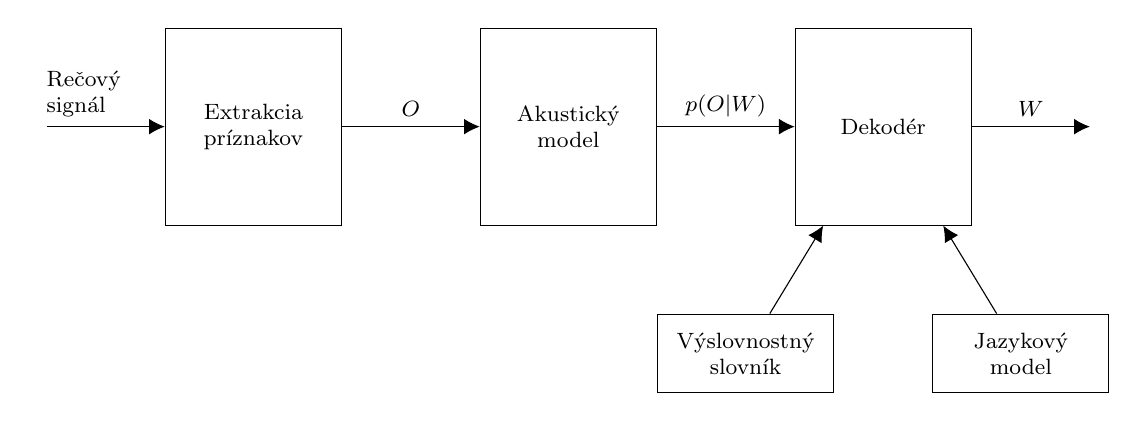
\begin{tikzpicture}[every node/.style = {font=\footnotesize}, node distance=4cm, >={Latex[width=2mm,length=2mm]}]
		\tikzstyle{block} = [rectangle, minimum width=2cm, minimum height=2.5cm, text centered, text width=2cm, draw=black]
		\tikzstyle{small block} = [block, minimum height=1cm]
		%\tikzstyle{arrow} = [thick,->,>=stealth]
		\tikzstyle{arrow} = [->]

		%\node[io](speech){Rečový signál};
		\node[block](fe){Extrakcia príznakov};
		\node[left=1.5cm of fe] (input) {};
		\node[block, right of=fe](am){Akustický model};
		\node[block, right of=am](decoder){Dekodér};
		\node[right=1.5cm of decoder](output) {};
		\node[below=1.5cm of decoder](dummy){};
	    \node[small block, left=0.5cm of dummy] (lexicon) {Výslovnostný slovník};
		\node[small block, right=0.5cm of dummy](lm){Jazykový model};

		\draw[arrow] (input) -- (fe) node[midway, above, text width=1.5cm, align=flush left] {Rečový signál};
		\draw[arrow] (fe) -- (am) node[midway, above] {$\bm{O}$};
		\draw[arrow] (am) -- (decoder) node[midway, above] {$p(\bm{O}|W)$};
		\draw[arrow] (lexicon) -- (decoder);
		\draw[arrow] (lm) -- (decoder);
		\draw[arrow] (decoder) -- (output) node[midway, above] {$W$};
        %\node[io, text centered, above=0.5cm of am] (am-input) {KANONICKÝ PREPIS};
        %\node[io, right=0.5cm of am] (am-output) {FONÉMOVÉ ZAROVNANIA};
        %\node[below=0.5cm of am] (dummy) {};
       % \node[block, below=0.5cm of dummy] (fe) {EXTRAKCIA PRÍZNAKOV};
        %\node[io, right=0.5cm of fe] (fe-output) {PRÍZNAKY};
        %\node[block, right=7cm of dummy] (md) {DETEKCIA NESPRÁVNEJ VÝSLOVNOSTI};
        %\draw[arrow] (am) -- (am-output);
        %\draw[arrow] (am-input) -- (am);
        %\draw[arrow] (am-output) -| (md);
        %\draw[arrow] (fe) -- (fe-output);
        %\draw[arrow] (fe-output) -| (md);
\end{tikzpicture}

\ifstandalone
\end{document}
\fi